% DSCI 498 draft report -- compile with pdfLaTeX + BibTeX (Overleaf default).
% Figures: figures/*.pdf, regenerated by scripts/report_figures.py (no simulation needed).
% Layout: single column ("onecolumn"), 1-inch margins (geometry), figure widths set per figure.
% Figures are drawn at the size they are printed (see scripts/report_figures.py), so widths of
% 0.45-0.6\linewidth keep figure text at about 8 pt; change "width=" below to rescale one figure.
\documentclass[conference,onecolumn,10pt]{IEEEtran}
\IEEEoverridecommandlockouts

\usepackage[letterpaper,margin=1in]{geometry}
\usepackage{microtype}
\usepackage{cite}
\usepackage{amsmath,amssymb}
\usepackage{graphicx}
\usepackage{booktabs}
\usepackage{xcolor}
\usepackage{url}
\usepackage[hidelinks]{hyperref}

\graphicspath{{figures/}}
\newcommand{\todo}[1]{\textcolor{red}{[TODO: #1]}}
\newcommand{\lime}{LIME-$\Delta$}
% Float placement: allow figures/tables to sit in the text instead of piling up at page tops.
\renewcommand{\topfraction}{0.85}
\renewcommand{\textfraction}{0.15}
\renewcommand{\floatpagefraction}{0.75}
\setlength{\textfloatsep}{10pt plus 2pt minus 2pt}
\setlength{\intextsep}{10pt plus 2pt minus 2pt}

\begin{document}

\title{Can a Troubleshooter Trust a Filter Surrogate's Explanation?\\
Faithfulness, Usefulness, and a Full-Wave Stress Test of SHAP, IG and LIME}

\author{\IEEEauthorblockN{\todo{author names}}
\IEEEauthorblockA{DSCI 498: Explainable AI, Lehigh University\\
Draft report, December 2, 2026}}

\maketitle

\begin{abstract}
We study whether explanations of a neural surrogate for a coupled-line microstrip band-pass filter can be trusted by a receive-side RF troubleshooter who must decide which failed specification to check and what to hand to the component designer.
The surrogate (PR-Net, a pole--residue network) is trained on 1440 ADS circuit simulations with six geometry inputs and three negative-control inputs.
We explain a reference-relative (contrastive) mask-violation target with exact SHAP, Integrated Gradients and a LIME-based contribution, and ask three questions.
\emph{True:} on a test set frozen before evaluation, SHAP attributions agree with ground-truth Shapley values computed in ADS (Spearman 0.98--0.99, sign agreement 1.00), and the residual disagreement of IG and LIME comes from the explainers, not from the network.
\emph{Useful:} in a pre-registered tuning experiment, changing only the two SHAP-ranked parameters fixed 25 of 30 failing designs versus 6 of 30 for random pairs; however, a plain six-parameter surrogate search fixed all 30, so the explanation's value lies in localization and hand-off rather than speed.
\emph{Hold up:} when three SHAP-tuned designs were re-simulated with an independent full-wave solver (openEMS), none passed the mask; two improved by about 13\,dB and one became worse.
Two full-wave solvers agree that the circuit model over-estimates bandwidth by about 0.13\,GHz and omits about 17\% passband radiation, which explains the failures.
A trust heuristic from prior filter work, SHAP--LIME agreement, barely predicted agreement with ground truth (Spearman 0.24 over 3120 cases).
\end{abstract}

\begin{IEEEkeywords}
explainable AI, SHAP, integrated gradients, LIME, faithfulness, surrogate model, microstrip filter, full-wave validation
\end{IEEEkeywords}

%======================================================================
\section{Introduction}
%======================================================================
Neural surrogates of microwave components replace minute-long simulations with millisecond predictions, and recent work has started to attach post-hoc explanations to them~\cite{suslova2026}.
Whether such explanations deserve trust depends on who uses them and for what decision.
Table~\ref{tab:frame} fixes the four elements of the project and the explanation principle, and the framing question follows from them:

\begin{quote}
\emph{For a receive-side RF troubleshooter deciding which failed specification and frequency region to check first and what to hand to the component designer, does an explanation built on the contrastive principle improve decision quality without losing faithfulness?}
\end{quote}

\begin{table}[htbp]
\centering
\caption{Project framework.}
\label{tab:frame}
\small
\begin{tabular}{p{0.16\linewidth}p{0.70\linewidth}}
\toprule
Data & 1440 ADS circuit simulations of a coupled-line microstrip band-pass filter; 6 geometry inputs + 3 planted negative controls; $S$-parameters 9--15\,GHz. \\
Model & PR-Net, a pole--residue neural surrogate (main); M1 black-box MLP and M0 (replication of~\cite{suslova2026}) as comparisons. \\
Stakeholder & Receive-side RF front-end evaluation/troubleshooting engineer (one interview) and practitioner sources~\cite{rs_evm,adi_an1354}. \\
Decision & Which failed specification and frequency region to examine first; what to hand to the component designer (a ranked geometry hypothesis, not a validated fix). \\
Principle & Contrastive (Lipton~\cite{lipton1990}): why does this design violate the mask \emph{rather than} behave like a known-good reference design? \\
Improve / keep & Improve decision quality (ADS-confirmed fixes per simulation, a proxy); keep faithfulness (to the model and to an ADS ground truth). \\
\bottomrule
\end{tabular}
\end{table}

We answer the three course questions with evidence of different strength:
(Q1) \emph{are the explanations true}---faithful to the model and to a simulator ground truth;
(Q2) \emph{are they useful}---measured by a pre-registered decision proxy and shaped by a practitioner interview;
(Q3) \emph{do they hold up}---when the circuit simulator that generated the training data is replaced by a full-wave electromagnetic solver.

\textbf{Contributions.}
(i) A ground-truth faithfulness test in which Shapley values are computed directly in the circuit simulator (64 coalitions per design) on a test set frozen before evaluation, allowing us to separate explainer error from model error.
(ii) A pre-registered, simulator-confirmed tuning experiment that compares explanation-guided decisions with random, sensitivity-based, ground-truth and explanation-free baselines, including an unfavourable baseline.
(iii) A full-wave stress test showing that a decision validated inside the circuit model does not transfer, together with a physical account of why.
(iv) A negative result for the SHAP--LIME agreement heuristic used in prior filter work~\cite{suslova2026}.

\textbf{What was written down before results.} Table~\ref{tab:prereg} lists each test, when its protocol or expectation was recorded, and the outcome. Where we could not prove that a protocol preceded its results, we say so.

\begin{table}[htbp]
\centering
\caption{Tests, the record written before results, and outcomes.}
\label{tab:prereg}
\small
\begin{tabular}{p{0.30\linewidth}p{0.30\linewidth}p{0.28\linewidth}}
\toprule
Test / expectation & Recorded before results & Outcome \\
\midrule
Negative controls: a model that ignores them should receive $\approx0$ attribution & Planted in the dataset; expectation in the analysis plan (Oct 24) & Supported (Sec.~\ref{sec:ground}) \\
Known answer: T0 ranking $L_2>L_1>W_{c2}$ & Analysis plan (Oct 24) & Supported by all methods \\
Explainer vs.\ ADS ground-truth Shapley; explainer/network/physics decomposition & Hash-frozen protocol, Oct 25 17:21 UTC, before any test label was read (no numeric threshold set) & SHAP 0.98--0.99; IG/LIME lower (Sec.~\ref{sec:truth}) \\
Explainer-selected parameter pairs fix more failing designs than random pairs & Pre-registration, Oct 25 19:23 UTC, before tuning code ran & Supported, $p_\text{Holm}=4\times10^{-5}$ (Sec.~\ref{sec:q2}) \\
Full-wave transfer of tuned designs & Case rule fixed in code before simulation; no expected outcome recorded & 0/3 pass (Sec.~\ref{sec:q3}) \\
Deletion/insertion vs.\ random orders & Described in the plan, but the pre-run version cannot be verified & Reported as supporting only \\
\bottomrule
\end{tabular}
\end{table}

%======================================================================
\section{Related Work}
%======================================================================
\textbf{Attribution methods.} SHAP~\cite{lundberg2017} allocates a prediction difference by the Shapley value~\cite{shapley1953}; Integrated Gradients~\cite{sundararajan2017} integrates gradients along a path from a baseline; LIME~\cite{ribeiro2016} fits a local surrogate.
All three require a reference or neighbourhood, which makes them inherently contrastive~\cite{lipton1990,miller2019} once the reference is stated.

\textbf{Evaluating faithfulness.} Deletion/insertion curves~\cite{petsiuk2018} and retrain-based removal~\cite{hooker2019} test whether high-attribution inputs matter to the model; randomization tests~\cite{adebayo2018} check that explanations depend on the model at all.
Jacovi and Goldberg~\cite{jacovi2020} separate faithfulness from plausibility; we add a third layer---agreement with the simulator that generated the labels---which is possible because the data come from a deterministic simulator in which Shapley values can be computed exactly.

\textbf{Explanations for microwave surrogates.} Suslova et al.~\cite{suslova2026} applied SHAP and LIME to neural models of microstrip filters and used SHAP--LIME agreement as evidence of reliable explanations; we replicate their network (M0) and test that heuristic against ground truth.
The gap between circuit and electromagnetic models is classical in microwave design and motivates space mapping~\cite{bandler1994}; we use it here as the ``unusual condition'' for Q3.

%======================================================================
\section{Stakeholder and Decision}
%======================================================================
Our stakeholder evidence is one semi-structured interview (internet voice call, November~5, 2026) with a practitioner who works on RF front-end evaluation and troubleshooting on the receive side of communication systems.
The notes are an edited paraphrase, not a verbatim transcript; the project had been introduced beforehand.
The practitioner treats the filter as a constraint on what reaches the receiver and does not edit microstrip geometry.
Typical problems (excess EVM, sensitivity loss, adjacent-channel interference) are narrowed by checking passband flatness, band edges and out-of-band rejection, then confirmed by measurement.
Practitioner sources agree that filter loss and rejection are only some of many contributors to such receiver-level symptoms~\cite{rs_evm,adi_an1354}, which is why the explanation must start from the failed filter specification rather than from the symptom.

Three requirements emerged and directly shaped our explanation design:
\textbf{(A) Specification first}---show the frequency region, the failed specification and the violation magnitude, in engineering units, before any attribution; a bare ranking such as ``L2 is important'' is not actionable.
\textbf{(B) Case-level quality}---an aggregate correlation does not say whether \emph{this} explanation is reliable.
\textbf{(C) Action boundary}---separate diagnostic attribution from a proposed parameter change, which needs separate validation.
Requirement (C) is why we evaluate tuning (Q2) and full-wave transfer (Q3) separately from faithfulness (Q1).
This is a single-person account; it constrains the design but is not evidence that the tool improves troubleshooting.

%======================================================================
\section{Data and Surrogate Models}
%======================================================================
\textbf{Data.} The dataset contains 1440 third-order coupled-line microstrip band-pass filters simulated in Keysight ADS (circuit level; substrate $H=15$\,mil, $\varepsilon_r=3.78$, lossless, ideal conductors), with $S_{21}$ and $S_{11}$ at 601 points from 9 to 15\,GHz.
Inputs are six geometry parameters (resonator lengths $L_1,L_2$, gaps $S_1,S_2$, widths $W_{c1},W_{c2}$, in mil) and three \emph{negative controls}---random columns that the simulator never sees.
The split is by design: 1008 train, 216 validation, 216 test.
The specification mask (Fig.~\ref{fig:case}) requires, in the passband 11.6--12.4\,GHz, $|S_{21}|\ge-0.5$\,dB and $|S_{11}|\le-10$\,dB; in 9--10.8\,GHz $|S_{21}|\le-20$\,dB; and in 13.2--15\,GHz $|S_{21}|\le-15$\,dB.
The hard \emph{mask violation} $V$ is the sum of the four worst-case exceedances in dB; $V=0$ means pass.

\textbf{Models.}
PR-Net maps the nine inputs to five conjugate pole pairs plus residues and evaluates $S_{21}$ and $S_{11}$ as a closed-form rational function, so its poles can be checked against vector-fitting ground truth~\cite{gustavsen1999}.
M1 is a frequency-conditioned MLP with the same complex output and no structural prior.
M0 reproduces the fully connected network of~\cite{suslova2026} and serves as a deliberately weaker model.
Each is trained with three seeds.
On the test set (Table~\ref{tab:acc}) PR-Net reaches 0.084\,dB $S_{21}$ MAE and 2.7\,MHz centre-frequency error, versus 1.11\,dB and 18\,MHz reported in~\cite{suslova2026}.

\begin{table}[htbp]
\centering
\caption{Test accuracy of the surrogates (216 designs, mean of 3 seeds).}
\label{tab:acc}
\small
\begin{tabular}{lcccc}
\toprule
Model & $S_{21}$ MAE (dB) & $S_{11}$ MAE (dB) & $f_0$ MAE (MHz) & BW $R^2$ \\
\midrule
PR-Net (main) & 0.084 & 0.078 & 2.73 & 0.910 \\
M1 (black box) & 0.021 & 0.025 & 0.37 & 1.000 \\
M0 (as in \cite{suslova2026}) & 0.266 & 0.811 & 29.3 & $-0.342$ \\
Reported in \cite{suslova2026} & 1.11 & -- & 18 & $-1.28$ \\
\bottomrule
\end{tabular}
\end{table}

%======================================================================
\section{Explanations and the Contrastive Principle}
%======================================================================
\textbf{Targets.} Attributions explain scalar functions of the predicted response:
T0 (spectral centroid, a known-answer check), T1 (point values of $S_{21}$/$S_{11}$),
T1b (mean passband $S_{21}$, the target of~\cite{suslova2026}),
T2 (smoothed passband ripple, worst passband return loss and mask violation; our main object), and T3 (resonator pole frequencies and $Q$, PR-Net only).
The smooth mask violation uses a log-sum-exp with temperature 0.05\,dB.

\textbf{Contrastive principle.} Following Lipton~\cite{lipton1990} and Miller~\cite{miller2019}, we explain a \emph{contrast}: why design $x$ violates the mask by $V(x)$ \emph{rather than} behaving like a fixed reference design $r$ (the ADS baseline geometry, controls at train mean).
This matches how the troubleshooter reasons---``what differs from a known-good unit?''---and gives every attribution a stated reference and unit, as Requirement~A demands.

\textbf{Methods.}
\emph{SHAP}~\cite{lundberg2017,shapley1953}: exact Shapley values of the single-reference game $v(S)=f(x_S,r_{\bar S})$, enumerating all $2^9=512$ coalitions, so there is no sampling error.
\emph{IG}~\cite{sundararajan2017}: path integral of gradients from $r$ to $x$ (256 steps).
\emph{LIME}~\cite{ribeiro2016}: local weighted linear fit around $x$; for comparison with additive methods we report \lime, the local slope times the displacement $x-r$, which is not an exact decomposition.
The methods answer different questions---reference-relative contribution, path-integrated sensitivity, local linear trend---so we expect principled disagreement on non-linear targets.

%======================================================================
\section{Q1: Are the Explanations True?}
%======================================================================
We separate two meanings of ``true''~\cite{jacovi2020}: faithful to the \emph{model}, and consistent with the \emph{simulator} that generated the data.

\subsection{Faithfulness to the model}
\label{sec:q1model}
\textbf{Internal checks.} SHAP additivity error is at most $1.6\times10^{-4}$.
IG completeness residual exceeds 1\% for 2.6\% of PR-Net entries overall but for 45\% of entries on the $S_{11}$ value at 12\,GHz, where the dB response passes near a log singularity; we treat this as a numerical failure mode, not a definitional disagreement.
LIME's held-out local $R^2$ has median 0.88 on T2, with 12\% of cases below 0.5.

\textbf{Deletion/insertion.} Following~\cite{petsiuk2018}, inputs are replaced by reference values in attribution order and the normalized area under the output curve is compared with 100 random orders.
On PR-Net T2 (40 validation designs), the SHAP order lies in the best 5\% of random orders for 80\% (deletion) and 89\% (insertion) of entries; IG 69\%/86\%; \lime{} 64\%/93\%.
With only nine, strongly ranked inputs this is an easy test, and we could not verify that its protocol was written before it was run, so we report it as supporting, not decisive, evidence.

\textbf{Negative controls.} With SHAP and IG, PR-Net assigns at most 1\% of total $|\phi|$ to the three controls (\lime: up to 4\%), matching its measured interventional sensitivity to them (0--1\%).
M0 assigns 3--7\% (SHAP), consistent with its actual sensitivity of 4--8\%: the explanation correctly exposes that the weaker model uses a spurious input~\cite{adebayo2018}.

\subsection{Where and why the three methods disagree}
\label{sec:disagree}
On PR-Net (validation, rank correlation of $|\phi|$ over nine inputs) the methods agree almost perfectly on the near-linear known-answer target T0 (SHAP--IG 0.99, SHAP--\lime{} 0.96) and diverge on the non-linear mask target T2 (0.93 and 0.85); a linear model explains only 13--23\% of the variance of the T2 targets.
We trace the disagreement to four sources:
\begin{enumerate}
\item \emph{Different questions.} SHAP averages marginal effects over all coalitions with the reference; IG follows one straight path; \lime{} extrapolates a local slope over the whole displacement. With interactions (e.g.\ between $L_1$ and $L_2$, which jointly set band position) these are different quantities, not noisy estimates of one.
\item \emph{Numerics.} IG violates completeness near $S_{11}$ notches (Sec.~\ref{sec:q1model}), where the dB target is nearly singular.
\item \emph{Locality.} Halving LIME's neighbourhood (0.5$\to$0.25) changes its T2 ranking (0.85), and a new sampling seed changes it further (0.91).
\item \emph{Reference.} SHAP with one reference vs.\ a 32-design background agrees only at 0.70--0.78; the ``contrast'' changes, so the answer changes.
\end{enumerate}
The ground truth in Sec.~\ref{sec:truth} settles which disagreement matters: SHAP's single-reference game is the same game the simulator truth uses, and it is the method that matches.

\subsection{Domain grounding: what the model should have learned}
\label{sec:ground}
We state four ground-truth expectations before checking them.
(i) \emph{Controls:} the simulator never reads the three control columns, so their true effect is exactly zero; PR-Net's explanations reflect this (above).
(ii) \emph{Known answer:} the spectral centroid T0 is set by the resonator lengths, so the ranking should be $L_2>L_1>W_{c2}\gg$ others; all four methods (SHAP, IG, LIME slope, gradient) recover it on PR-Net (rank correlation 0.94 with a train-set regression).
(iii) \emph{Filter physics:} resonator length should dominate band position and coupling gap should shape the response; the ADS ground truth for the mask violation ranks $L_2>L_1>S_2$ on both splits, and for the quality factor of the middle in-band pole it ranks coupling geometry first ($S_1>W_{c1}$), as expected for a coupling-controlled quantity.
(iv) \emph{Concepts:} PR-Net's internal pole frequencies and $Q$ (T3) can be checked against vector fitting~\cite{gustavsen1999} of the ADS responses; the model's finite-difference sensitivities of these concepts match the vector-fitted ADS ones (sign agreement 0.98, rank correlation 0.99), and SHAP on T3 matches the ADS Shapley values at 0.98.

\subsection{Consistency with a simulator ground truth}
\label{sec:truth}
\textbf{Protocol written before evaluation.} On October~25, 2026 (17:21 UTC), before any test label was read, we recorded SHA-256 hashes of 30 files (trained models, code, analysis plan) together with the evaluation protocol (Table~\ref{tab:prereg}); validation results had already been used for development; the data loader refuses to return test labels until that record exists.
For 80 designs (40 validation, 40 test) we simulated all $2^6=64$ geometry coalitions of the same single-reference game directly in ADS, giving exact ground-truth Shapley values for every target.
The full coalition reproduces the dataset exactly (max $|\Delta S|=0$).

\textbf{Result.} Fig.~\ref{fig:decomp} decomposes agreement into \emph{network vs.\ ADS} (does the model's own game match physics?) and \emph{explainer vs.\ ADS}.
For PR-Net the network game agrees with ADS at Spearman 0.98--0.99 on every target; SHAP inherits this (0.98--0.99, sign agreement 1.00), while IG falls to 0.82 and \lime{} to 0.84 on T2.
Because SHAP vs.\ network is 0.99, the IG/LIME gap is explainer error, not model error.
For M0 the network itself agrees with ADS at only 0.80--0.91; SHAP tracks the network (0.81--0.92), while IG and \lime{} lose up to a further 0.05.
A naive explanation from train-set linear regression reaches only 0.56--0.59 on T1b/T2, so the model-based explanations add real information.

\begin{figure}[htbp]
\centering
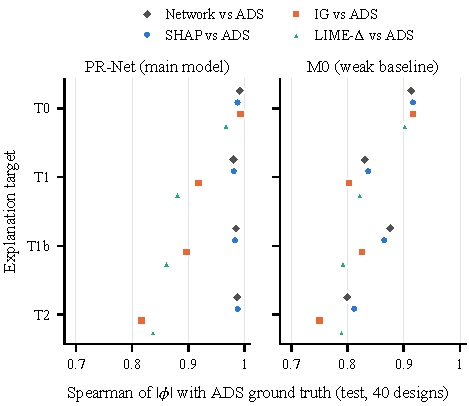
\includegraphics[width=0.55\linewidth]{fig_decomposition.pdf}
\caption{Agreement of attribution magnitudes with ADS ground-truth Shapley values (test). ``Network vs ADS'' compares the model's own game with the simulator; explainer points below it are explainer error.}
\label{fig:decomp}
\end{figure}

\textbf{A trust heuristic that fails.} Prior work~\cite{suslova2026} reads SHAP--LIME rank agreement as a sign of trustworthy explanations.
Across 3120 (design, target) pairs, this agreement predicts agreement with ADS ground truth at Spearman only 0.24 (0.20--0.24 per model under the original protocol; 0.12--0.15 for PR-Net and M1, 0.47 for M0, when SHAP and \lime{} use the same single-reference game as the ground truth).
Explainer agreement is therefore not a usable proxy for correctness here.

%======================================================================
\section{Q2: Are the Explanations Useful?}
\label{sec:q2}
%======================================================================
We have no user study; Q2 rests on a decision proxy and on the interview.
The proxy models Requirement~C's hand-off: if an attribution is offered to a designer as ``these two parameters cause the violation'', does acting on it fix the design?

\textbf{Pre-registered experiment.} Before running any tuning code we wrote down cases, selectors, search and statistics with a UTC timestamp and plan hash.
Thirty failing single-band test designs were drawn with a fixed seed.
Each selector picks two of the six geometry parameters; a PR-Net search inside that two-dimensional box (41$\times$41 grid plus projected Adam, objective = smooth violation with a safety margin + a small move penalty) proposes a design, and ADS confirms it.
Up to ten ADS calls are allowed per case, the margin growing by 0.25\,dB after each failed call; success means ADS hard violation $V=0$.
The primary test is exact McNemar of each explainer versus random pairs, Holm-corrected.

\begin{figure}[htbp]
\centering
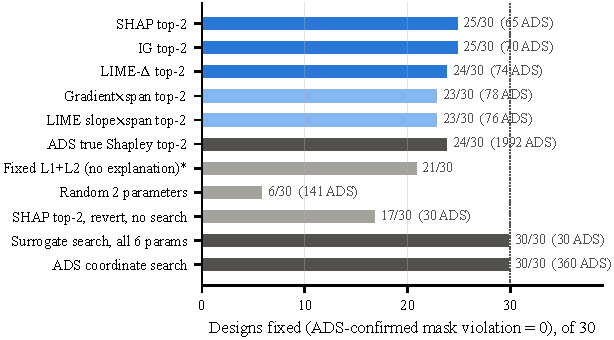
\includegraphics[width=0.6\linewidth]{fig_tuning.pdf}
\caption{Pre-registered tuning on 30 failing test designs (PR-Net surrogate, ADS confirmation). Blue: explanation-selected pairs; light blue: sensitivity baselines; dark: references; gray: baselines. Totals in brackets are ADS calls (ground-truth Shapley includes 64 coalition simulations per case). *Exploratory, not pre-registered.}
\label{fig:tuning}
\end{figure}

\textbf{Result} (Fig.~\ref{fig:tuning}).
SHAP-selected pairs fixed 25/30 designs versus 6/30 for random pairs (20 vs.\ 1 discordant cases, McNemar $p_{\text{Holm}}=4.2\times10^{-5}$; median paired reduction of the best ADS violation versus random 4.5\,dB, Wilcoxon $p_{\text{Holm}}=4.2\times10^{-5}$); IG 25/30 and \lime{} 24/30 were equally significant.
SHAP chose the same pair as the ADS ground truth in 87\% of cases at 1/30 of the simulation cost.
Two baselines temper this result.
A six-parameter surrogate search \emph{without any explanation} fixed all 30 designs with a single ADS call each, and always tuning $L_1$+$L_2$ fixed 21/30.
Reverting the SHAP-top-2 parameters to the reference without searching fixed only 17/30: the explanation names \emph{where} to act but not \emph{how much}.
In an exploratory rerun with the weaker M0 as surrogate, SHAP still fixed 22/30, so the benefit degrades gracefully with model quality.

\textbf{Interpretation for the stakeholder.} Explanations do not make tuning faster than optimization; their value is in localization and communication---telling the troubleshooter which specification and region failed, and giving the designer a ranked, simulator-consistent hypothesis.
Table~\ref{tab:card} shows the case summary we propose, ordered by Requirements A--C.
Whether it improves a real decision remains untested \todo{follow-up session with the practitioner on this card}.

\begin{table}[htbp]
\centering
\caption{Proposed specification-first case summary (test\_0005).}
\label{tab:card}
\small
\begin{tabular}{p{0.13\linewidth}p{0.68\linewidth}}
\toprule
A. Failure & Passband 11.6--12.4\,GHz: $|S_{11}|$ exceeds $-10$\,dB by 6.1\,dB; $|S_{21}|$ below $-0.5$\,dB by 1.8\,dB. Total $V=7.9$\,dB. Stopbands pass. \\
B. Quality & SHAP exact (additivity $<10^{-3}$); surrogate error at $x_0$ (median over cases 0.06\,dB). \todo{per-case LIME $R^2$, IG residual} \\
C. Diagnosis & Relative to the reference design, $L_1$ and $S_2$ contribute most to $V$ (SHAP). \\
C. Proposal & Change $L_1$ +7.2\,mil, $S_2$ +0.6\,mil: passes in ADS circuit model. \textbf{Not validated in full-wave}: fails by 10.2\,dB in openEMS (Sec.~\ref{sec:q3}). \\
\bottomrule
\end{tabular}
\end{table}

%======================================================================
\section{Q3: Do the Decisions Hold Up Under a Change of Physics Model?}
\label{sec:q3}
%======================================================================
The ADS labels are circuit-level: coupled-line models without radiation or full electromagnetic coupling.
We originally planned a few HFSS checks; without a licence we used the open-source FDTD solver openEMS~\cite{liebig2013} (v0.37) on the identical layout as the dataset's Momentum diagnostic template (zero-thickness PEC, same lossless substrate, 50\,$\Omega$ microstrip ports, 601 frequency points).

\textbf{Calibration.} Mesh refinement on the baseline (Fig.~\ref{fig:mesh}) moves the openEMS centre frequency \emph{up} (11.89$\to$12.03\,GHz; last step 22\,MHz) while Momentum moves \emph{down} (12.18$\to$12.13\,GHz), bracketing the ADS value of 12.05\,GHz.
Thus part of the 124\,MHz Momentum--circuit offset documented with the dataset is a Momentum mesh artefact.
Both full-wave solvers agree on a narrower bandwidth (openEMS 1.16, Momentum 1.13, ADS 1.29\,GHz) and on about 17--18\% of power not returned to either port in the passband ($1-|S_{11}|^2-|S_{21}|^2$, ADS: 0), i.e.\ radiation worth about 0.8\,dB of insertion loss.
The finest openEMS mesh (3.8\,M cells, about 13\,min per run) was used for all cases.

\textbf{Case rule.} Walking the 30 pre-registered cases in order, we kept those where SHAP tuning succeeded in ADS and whose SHAP pair had not been used, stopping at three (test\_0005: $L_1,S_2$; test\_0015: $L_1,L_2$; test\_0034: $L_2,S_1$).
The rule was fixed in code before any case was simulated, but was not externally time-stamped.
Each original design $x_0$ and its SHAP-tuned design were simulated.

\textbf{Result.} None of the three tuned designs passes in full-wave (Fig.~\ref{fig:fw}, Table~\ref{tab:fw}).
For test\_0015 and test\_0034 the decision \emph{direction} transfers: violation drops by 13.5 and 13.4\,dB.
For test\_0005 it reverses: violation rises from 6.4 to 10.2\,dB.
These verdicts are robust to the mesh: the last refinement changed the baseline violation by only 0.12\,dB.

\begin{figure}[htbp]
\centering
\begin{minipage}[t]{0.48\linewidth}
\centering
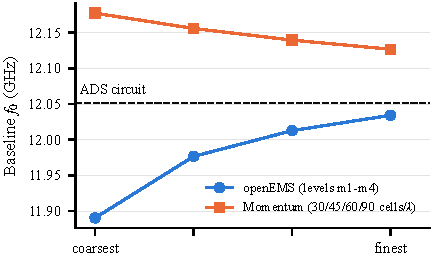
\includegraphics[width=\linewidth]{fig_mesh.pdf}
\caption{Baseline centre frequency under mesh refinement. The two full-wave solvers converge from opposite sides towards the circuit value.}
\label{fig:mesh}
\end{minipage}\hfill
\begin{minipage}[t]{0.48\linewidth}
\centering
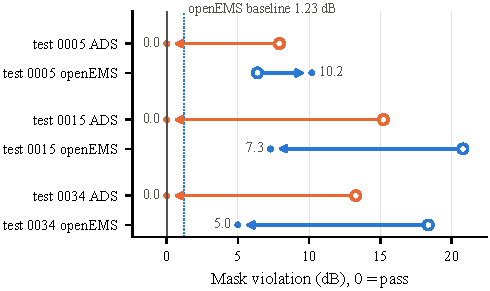
\includegraphics[width=\linewidth]{fig_fullwave_summary.pdf}
\caption{Mask violation before (hollow) and after (filled) SHAP-guided tuning, in ADS and in openEMS. Dotted: untouched baseline in openEMS.}
\label{fig:fw}
\end{minipage}
\end{figure}

\begin{table}[htbp]
\centering
\caption{Full-wave check of SHAP-tuned designs (openEMS, finest mesh). Shift = openEMS $-$ ADS for the tuned design.}
\label{tab:fw}
\small
\begin{tabular}{lccccc}
\toprule
Design & $V_\text{ADS}$ & $V_\text{oEMS}$ & $V_\text{oEMS}$ & $f_0$ shift & BW shift \\
 & $x_0\to$ tuned & $x_0$ & tuned & (MHz) & (MHz) \\
\midrule
test\_0005 & 7.9 $\to$ 0 & 6.4 & 10.2 & $-49$ & $-124$ \\
test\_0015 & 15.2 $\to$ 0 & 20.8 & 7.3 & $-49$ & $-129$ \\
test\_0034 & 13.3 $\to$ 0 & 18.4 & 5.0 & $-53$ & $-142$ \\
\bottomrule
\end{tabular}
\end{table}

\textbf{Mechanism.} The pre-registered search stops at the first ADS pass, so tuned designs sit on the mask edge with almost no margin.
The full-wave response is 0.12--0.14\,GHz narrower and 50\,MHz lower than the circuit response, which pushes each edge design into passband $S_{21}$, passband $S_{11}$ and low-stopband violations (the high stopband never fails).
test\_0005 (Fig.~\ref{fig:case}) is instructive: its original failure was matching ($S_{11}$), with a well-centred passband (12.05\,GHz).
The SHAP pair $L_1,S_2$ repaired it in ADS by moving the centre frequency down 141\,MHz---a path that is valid in the circuit model but runs in the same direction as the circuit-to-full-wave shift, adding a 3.3\,dB low-stopband violation in full-wave.
The attribution was faithful to the model it explained; the \emph{decision} built on it inherited that model's systematic error.

\begin{figure}[htbp]
\centering
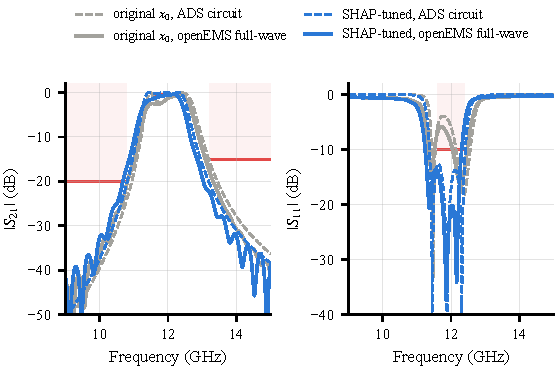
\includegraphics[width=0.6\linewidth]{fig_fullwave_case.pdf}
\caption{test\_0005 before (gray) and after (blue) SHAP-guided tuning; dashed: ADS circuit, solid: openEMS full-wave. Red segments: mask limits; shaded: forbidden regions. The tuned design passes in ADS but moves into the low stopband in full-wave.}
\label{fig:case}
\end{figure}

%======================================================================
\section{Failed or Abandoned Explanations}
%======================================================================
\begin{itemize}
\item \textbf{SHAP--LIME agreement as a trust signal} (Sec.~\ref{sec:truth}): barely predicts ground-truth agreement (Spearman 0.24 overall). Abandoned as a quality indicator for Requirement~B.
\item \textbf{IG on $S_{11}$ notches}: 45\% of entries violate completeness by more than 1\% even with 256 steps. IG is not shown to the stakeholder for $S_{11}$ targets.
\item \textbf{SHAP read as local sensitivity}: at the baseline, SHAP magnitudes (distributional background) agree with ADS single-parameter perturbations at Spearman only 0.33, whereas gradient$\times$span reaches 0.58 and model finite differences 0.98. SHAP answers a contrastive question, not ``which knob is most sensitive here''.
\item \textbf{Background dependence}: single-reference SHAP and SHAP with a 32-point background agree only at 0.70--0.78; the reference must always be stated.
\item \textbf{Attribution as a step size}: reverting the top-2 SHAP parameters to the reference fixed only 17/30 designs.
\item \textbf{Tuning advice across models}: 0/3 SHAP-tuned designs pass in full-wave (Sec.~\ref{sec:q3}).
\item \textbf{Abandoned framing}: we first framed the stakeholder as a filter designer choosing which two dimensions to tune. The only practitioner available does not edit geometry, so the decision was re-framed to troubleshooting and hand-off.
\end{itemize}

%======================================================================
\section{Limitations}
%======================================================================
Stakeholder evidence is a single paraphrased interview; Q2 is a simulator proxy, not a user study.
The full-wave check covers three designs and shows a clear counter-example with a consistent mechanism, not a failure rate.
openEMS is not HFSS and shows extra non-physical loss out of band (12\% at 9\,GHz versus 2\% for Momentum), visible as ripple below $-30$\,dB; it does not affect mask verdicts, but out-of-band details should not be read from it.
Both simulators assume ideal conductors and a lossless substrate; adding loss would only worsen the passband.
Ground-truth Shapley values are defined for one reference; other references can rank parameters differently.

%======================================================================
\section{Conclusion}
%======================================================================
For the troubleshooter's decision, the answer to our framing question is split.
The contrastive SHAP explanation is \emph{true}: faithful to the network and, through it, to the circuit simulator, with errors that we can attribute to explainer or model.
It is \emph{useful} as localization and as a ranked hypothesis to hand to a designer, but not as a faster tuning method.
It does \emph{not hold up} as tuning advice when the physics changes: a design that the explanation helped to fix in the circuit model failed in full-wave in all three cases checked, and got worse in one.
The practical rule we would give the stakeholder is therefore Requirement~C made concrete: treat attribution as diagnosis, and treat any explanation-guided design change as unvalidated until it has margin for a $\sim$0.13\,GHz bandwidth loss and $\sim$50\,MHz shift, or has passed a full-wave check.

\todo{Final version: repository link, README, decision log, AI-use reflection (separate document).}

\bibliographystyle{IEEEtran}
\bibliography{references}

\end{document}
